\documentclass[a4paper]{article}
\usepackage{fontspec}
\setmainfont{Linux Libertine O}[Scale=MatchLowercase]
\usepackage{xeCJK}
\setCJKmainfont{NotoSansCJK-Regular.ttc}[
	Path = /usr/share/fonts/noto/,
]
% \usepackage[absolute,noshowtext,showboxes]{textpos}
\usepackage[absolute,showboxes]{textpos}
% \textblockorigin{-0.02cm}{0.07cm} %HPDeskJet5160
% \textblockorigin{0.00cm}{0.00cm} %HPDeskJet5160
\textblockorigin{0.00cm}{0.00cm} %HPDeskJet5160
% \textblockorigin{0.05cm}{0.13cm} %HPDeskJet5160
% \textblockorigin{0.00cm}{0.00cm} %HPLaserJet5000LE
\usepackage{graphicx}
\graphicspath{ {/home/$ENV{USER}/ttb/trunk/forms/bean/} }
\pagestyle{empty}
\setlength{\unitlength}{1cm}

\setlength{\TPVertModule}{1.6875cm}

\newcommand{\myXfourthreetwoBeanXIdentifier}[0]{
seventeen bean
}

\newcommand{\myXfourBean}[0]{
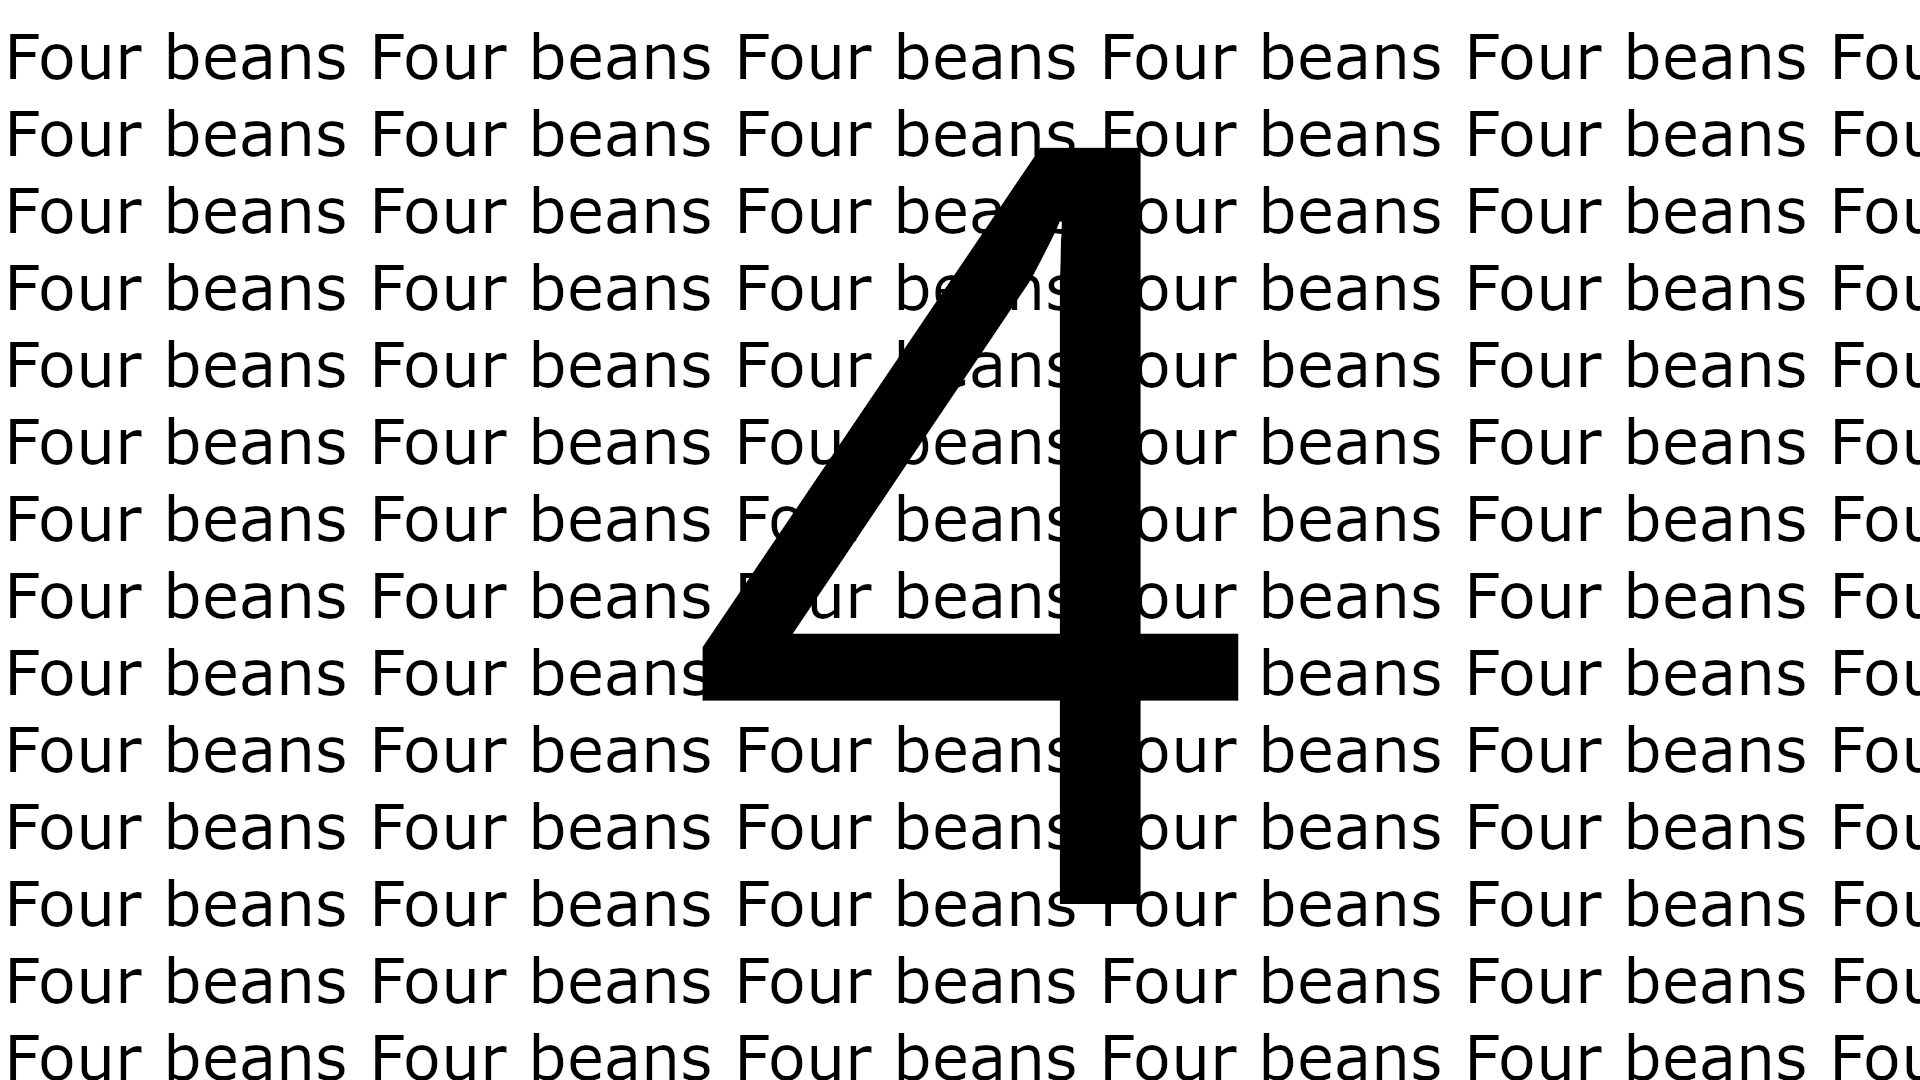
\includegraphics[angle=90,height=0.057\paperheight,width=0.150\paperwidth]{four_bean.png}
}

\newcommand{\myXthreeBean}[0]{
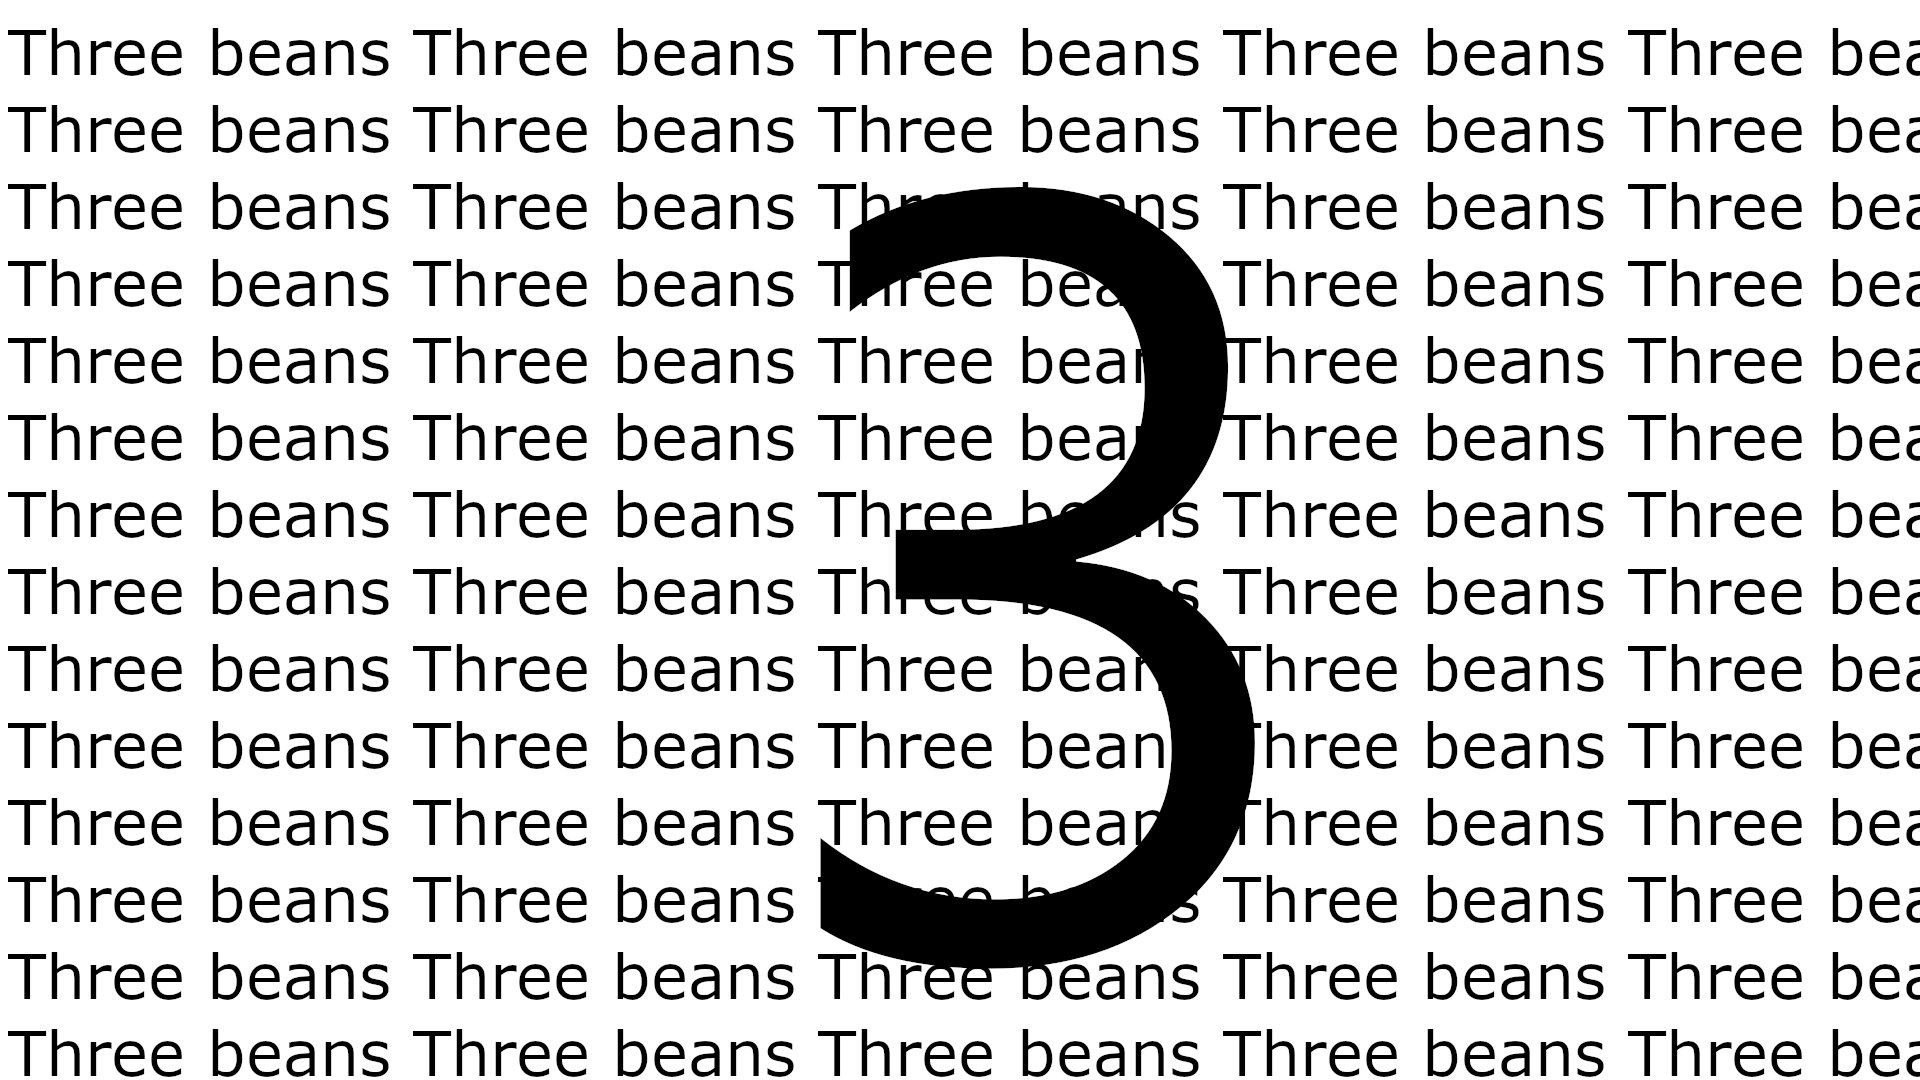
\includegraphics[angle=90,height=0.057\paperheight,width=0.150\paperwidth]{three_bean.png}
}

\newcommand{\myXtwoBean}[0]{
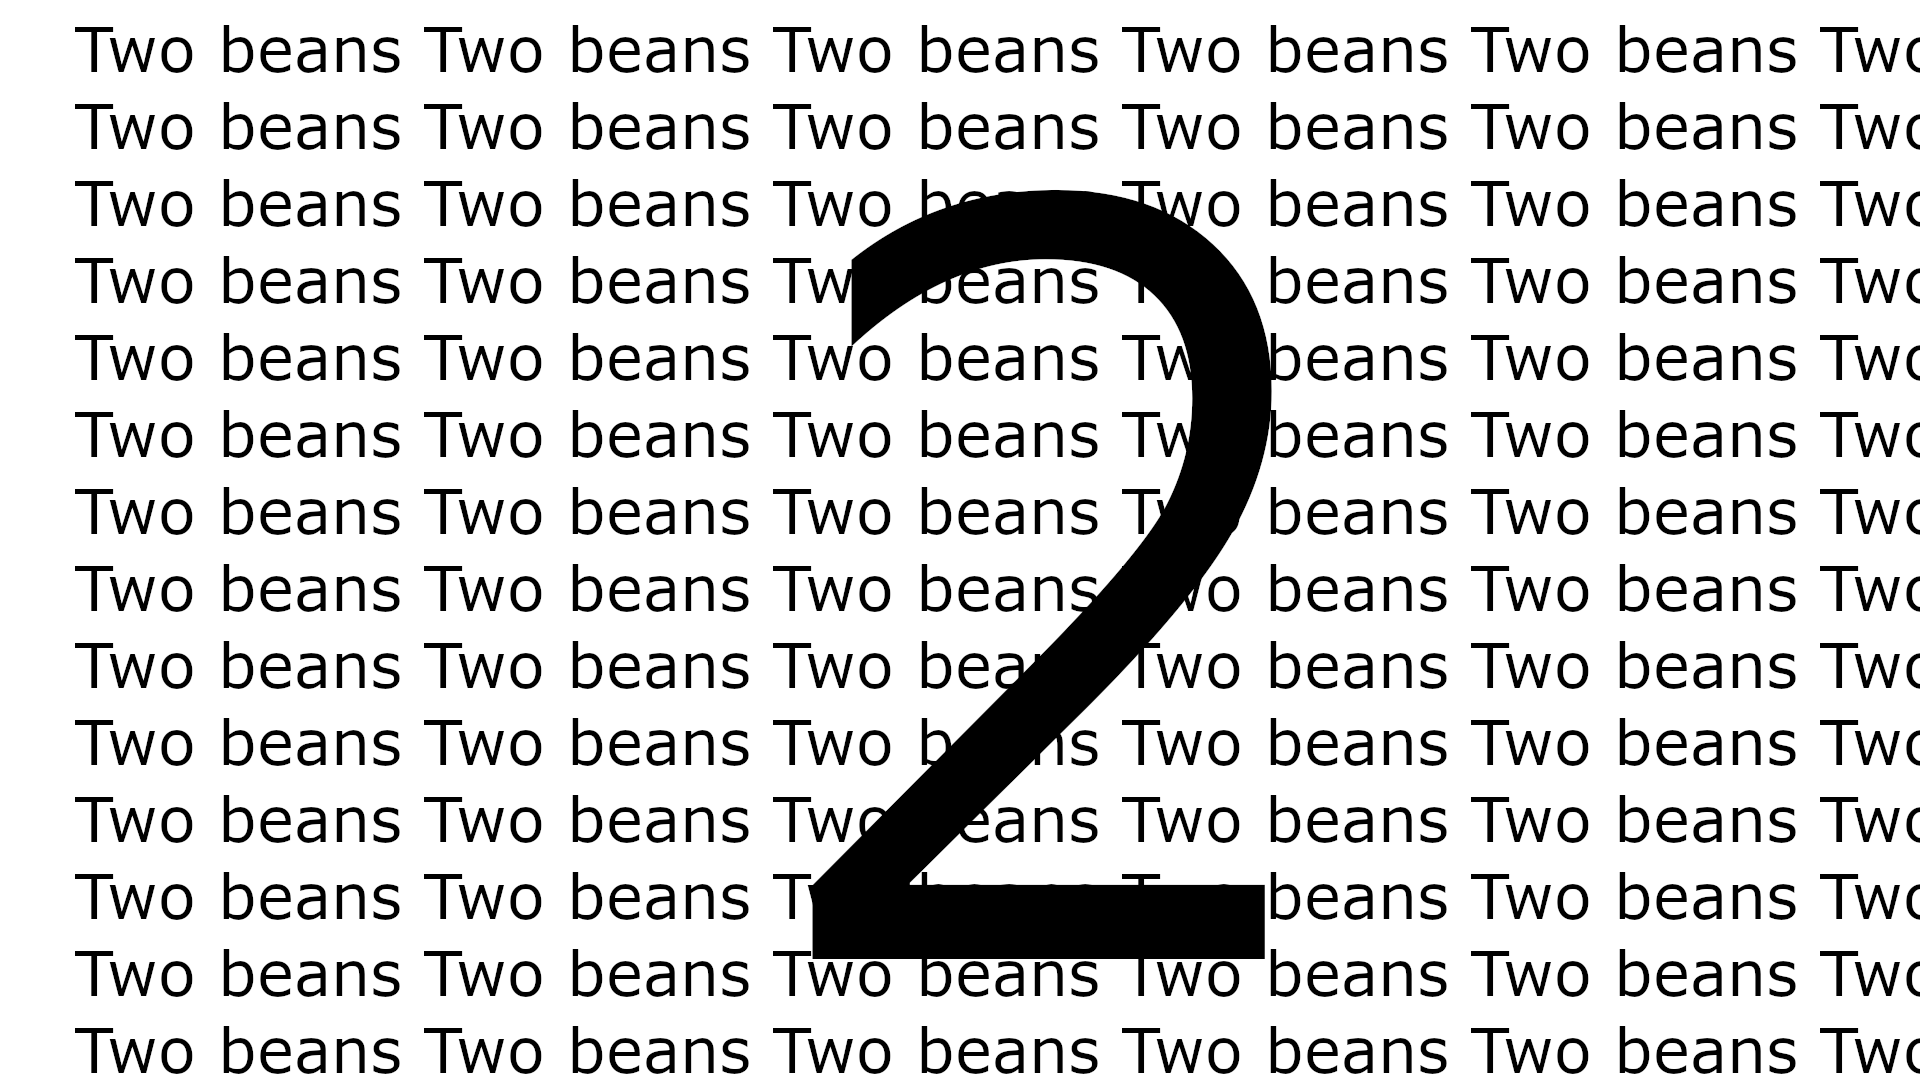
\includegraphics[angle=90,height=0.057\paperheight,width=0.150\paperwidth]{two_bean.png}
}

% \newcommand{\myDcontent}[0]{
% 
% }

\newcommand{\mycard}[5]{%
	\vspace{0.35cm}
	\tiny #1 #2
	% \vspace{-0.03cm}
	% \par
	\parbox[t][2.29\TPVertModule][c]{0.150\paperwidth}{%
	\hspace{-0.65cm} \large#3\\
	}
}

\begin{document}
% \begin{picture}(15,20)(+4.8,-22.05)
% \begin{tabular}[t]{*{2}{|p{10.05cm}}|}

% top line

\begin{textblock}{2.29}(0,0)
\textblocklabel{picture1}
\mycard{}{}{
\myXfourBean
}{}{} 
\end{textblock}

\begin{textblock}{2.29}(2.29,0)
\textblocklabel{picture1}
\mycard{}{}{
\myXfourBean
}{}{} 
\end{textblock}

\begin{textblock}{2.29}(4.57,0)
\textblocklabel{picture2}
\mycard{}{}{
\myXfourBean
}{}{} 
\end{textblock}

\begin{textblock}{2.29}(6.86,0)
\textblocklabel{picture2}
\mycard{}{}{
\myXfourBean
}{}{} 
\end{textblock}

\begin{textblock}{2.29}(9.14,0)
\textblocklabel{picture2}
\mycard{}{}{
\myXfourBean
}{}{} 
\end{textblock}

\begin{textblock}{2.29}(11.42,0)
\textblocklabel{picture3}
\mycard{}{}{
\myXfourBean
}{}{} 
\end{textblock}

\begin{textblock}{2.29}(13.71,0)
\textblocklabel{picture3}
\mycard{}{}{
\myXfourBean
}{}{} 
\end{textblock}

% second line

\begin{textblock}{2.29}(0,2.29)
\textblocklabel{picture1}
\mycard{}{}{
\myXfourBean
}{}{} 
\end{textblock}

\begin{textblock}{2.29}(2.29,2.29)
\textblocklabel{picture1}
\mycard{}{}{
\myXfourBean
}{}{} 
\end{textblock}

\begin{textblock}{2.29}(4.57,2.29)
\textblocklabel{picture2}
\mycard{}{}{
\myXfourBean
}{}{} 
\end{textblock}

\begin{textblock}{2.29}(6.86,2.29)
\textblocklabel{picture2}
\mycard{}{}{
\myXfourBean
}{}{} 
\end{textblock}

\begin{textblock}{2.29}(9.14,2.29)
\textblocklabel{picture2}
\mycard{}{}{
\myXfourBean
}{}{} 
\end{textblock}

\begin{textblock}{2.29}(11.42,2.29)
\textblocklabel{picture3}
\mycard{}{}{
\myXfourBean
}{}{} 
\end{textblock}

\begin{textblock}{2.29}(13.71,2.29)
\textblocklabel{picture3}
\mycard{}{}{
\myXfourBean
}{}{} 
\end{textblock}

% third line

\begin{textblock}{2.29}(0,4.57)
\textblocklabel{picture1}
\mycard{}{}{
\myXthreeBean
}{}{} 
\end{textblock}

\begin{textblock}{2.29}(2.29,4.57)
\textblocklabel{picture1}
\mycard{}{}{
\myXthreeBean
}{}{} 
\end{textblock}

\begin{textblock}{2.29}(4.57,4.57)
\textblocklabel{picture2}
\mycard{}{}{
\myXthreeBean
}{}{} 
\end{textblock}

\begin{textblock}{2.29}(6.86,4.57)
\textblocklabel{picture2}
\mycard{}{}{
\myXthreeBean
}{}{} 
\end{textblock}

\begin{textblock}{2.29}(9.14,4.57)
\textblocklabel{picture2}
\mycard{}{}{
\myXthreeBean
}{}{} 
\end{textblock}

\begin{textblock}{2.29}(11.42,4.57)
\textblocklabel{picture3}
\mycard{}{}{
\myXthreeBean
}{}{} 
\end{textblock}

\begin{textblock}{2.29}(13.71,4.57)
\textblocklabel{picture3}
\mycard{}{}{
\myXthreeBean
}{}{} 
\end{textblock}

% 4th line

\begin{textblock}{2.29}(0,6.86)
\textblocklabel{picture1}
\mycard{}{}{
\myXthreeBean
}{}{} 
\end{textblock}

\begin{textblock}{2.29}(2.29,6.86)
\textblocklabel{picture1}
\mycard{}{}{
\myXthreeBean
}{}{} 
\end{textblock}

\begin{textblock}{2.29}(4.57,6.86)
\textblocklabel{picture2}
\mycard{}{}{
\myXthreeBean
}{}{} 
\end{textblock}

\begin{textblock}{2.29}(6.86,6.86)
\textblocklabel{picture2}
\mycard{}{}{
\myXthreeBean
}{}{} 
\end{textblock}

\begin{textblock}{2.29}(9.14,6.86)
\textblocklabel{picture2}
\mycard{}{}{
\myXthreeBean
}{}{} 
\end{textblock}

\begin{textblock}{2.29}(11.42,6.86)
\textblocklabel{picture3}
\mycard{}{}{
\myXthreeBean
}{}{} 
\end{textblock}

\begin{textblock}{2.29}(13.71,6.86)
\textblocklabel{picture3}
\mycard{}{}{
\myXthreeBean
}{}{} 
\end{textblock}

% 5th line

\begin{textblock}{2.29}(0,9.14)
\textblocklabel{picture1}
\mycard{}{}{
\myXthreeBean
}{}{} 
\end{textblock}

\begin{textblock}{2.29}(2.29,9.14)
\textblocklabel{picture1}
\mycard{}{}{
\myXthreeBean
}{}{} 
\end{textblock}

\begin{textblock}{2.29}(4.57,9.14)
\textblocklabel{picture2}
\mycard{}{}{
\myXthreeBean
}{}{} 
\end{textblock}

\begin{textblock}{2.29}(6.86,9.14)
\textblocklabel{picture2}
\mycard{}{}{
\myXthreeBean
}{}{} 
\end{textblock}

\begin{textblock}{2.29}(9.14,9.14)
\textblocklabel{picture2}
\mycard{}{}{
\myXthreeBean
}{}{} 
\end{textblock}

\begin{textblock}{2.29}(11.42,9.14)
\textblocklabel{picture3}
\mycard{}{}{
\myXthreeBean
}{}{} 
\end{textblock}

\begin{textblock}{2.29}(13.71,9.14)
\textblocklabel{picture3}
\mycard{}{}{
\myXthreeBean
}{}{} 
\end{textblock}

% 6th line

\begin{textblock}{2.29}(0,11.42)
\textblocklabel{picture1}
\mycard{}{}{
\myXtwoBean
}{}{} 
\end{textblock}

\begin{textblock}{2.29}(2.29,11.42)
\textblocklabel{picture1}
\mycard{}{}{
\myXtwoBean
}{}{} 
\end{textblock}

\begin{textblock}{2.29}(4.57,11.42)
\textblocklabel{picture2}
\mycard{}{}{
\myXtwoBean
}{}{} 
\end{textblock}

\begin{textblock}{2.29}(6.86,11.42)
\textblocklabel{picture2}
\mycard{}{}{
\myXtwoBean
}{}{} 
\end{textblock}

\begin{textblock}{2.29}(9.14,11.42)
\textblocklabel{picture2}
\mycard{}{}{
\myXtwoBean
}{}{} 
\end{textblock}

\begin{textblock}{2.29}(11.42,11.42)
\textblocklabel{picture3}
\mycard{}{}{
\myXtwoBean
}{}{} 
\end{textblock}

\begin{textblock}{2.29}(13.71,11.42)
\textblocklabel{picture3}
\mycard{}{}{
\myXtwoBean
}{}{} 
\end{textblock}

% 7th line

\begin{textblock}{2.29}(0,13.71)
\textblocklabel{picture1}
\mycard{}{}{
\myXtwoBean
}{}{} 
\end{textblock}

\begin{textblock}{2.29}(2.29,13.71)
\textblocklabel{picture1}
\mycard{}{}{
\myXtwoBean
}{}{} 
\end{textblock}

\begin{textblock}{2.29}(4.57,13.71)
\textblocklabel{picture2}
\mycard{}{}{
\myXtwoBean
}{}{} 
\end{textblock}

\begin{textblock}{2.29}(6.86,13.71)
\textblocklabel{picture2}
\mycard{}{}{
\myXtwoBean
}{}{} 
\end{textblock}

\begin{textblock}{2.29}(9.14,13.71)
\textblocklabel{picture2}
\mycard{}{}{
\myXtwoBean
}{}{} 
\end{textblock}

\begin{textblock}{2.29}(11.42,13.71)
\textblocklabel{picture3}
\mycard{}{}{
\myXtwoBean
}{}{} 
\end{textblock}

\begin{textblock}{2.29}(13.71,13.71)
\textblocklabel{picture3}
\mycard{}{}{
\myXtwoBean
}{}{} 
\end{textblock}

% 8th line

% 9th line

% 10th line

% 11th line

% 12th line

% 13th line

% 14th line

% 15th line

\begin{tiny}1\end{tiny}\newpage;

% top line

% second line

% third line

% 4th line

% 5th line

% 6th line

% 7th line

% 8th line

% 9th line

% 10th line

% 11th line

% 12th line

% 13th line

% 14th line

% 15th line

\begin{tiny}2\end{tiny};

\end{document}
